\documentclass[10pt]{article}
\usepackage[margin=0.5in]{geometry}
\usepackage{multicol}
\usepackage{lipsum}% dummy text
\usepackage{amsmath}
\usepackage[compact]{titlesec}
\usepackage{graphicx}

\setlength{\columnseprule}{0pt}
\setlength{\parskip}{0pt}
\setlength{\parindent}{0pt} 
\setlength\abovedisplayskip{0pt}
\setlength\belowdisplayskip{0pt}
\setlength{\jot}{0pt}
\linespread{0.9}

\allowdisplaybreaks

\begin{document}
\begin{multicols}{3}

    \section*{Test 1}
    \subsection*{asdfasd}
    asdfasdfasdf
    \subsection*{asdfasd}
    asdfasdfasdf
    \subsection*{asdfasd}
    asdfasdfasdf

    \section*{Test 2}
    \subsection*{asdfasd}
    asdfasdfasdf
    \subsection*{asdfasd}
    asdfasdfasdf
    \subsection*{asdfasd}
    asdfasdfasdf

    \section*{General}
    \subsection*{Demorgans Law}
    \begin{align}
        \neg[p\wedge q]\equiv\neg p\vee\neg q,\\
        \neg[p\vee q]\equiv\neg p\wedge\neg q.
    \end{align}

    \subsection*{Gates}
    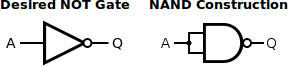
\includegraphics[width=\linewidth]{not.png}
    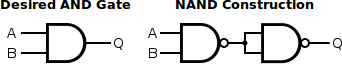
\includegraphics[width=\linewidth]{and.png}
    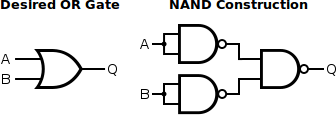
\includegraphics[width=\linewidth]{or.png}
    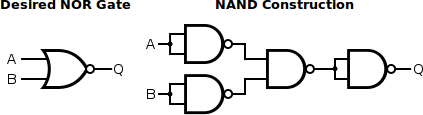
\includegraphics[width=\linewidth]{nor.png}
    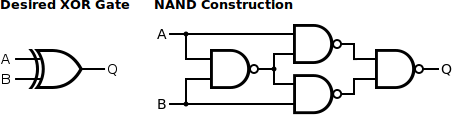
\includegraphics[width=\linewidth]{xor.png}

    \subsection*{Definitions}
    \textbf{Inertial Delay -} time it takes for signal to change value \\
    \textbf{Transport Delay -} time it takes for signal to travel down wire \\
    \textbf{Delta Cycle -} concept used to order vents that happen
    simultaneously \\
    \textbf{Channel Length Modulation -} shorting of the length of the inverted
    channel region with increase in drain bias for large drain biases \\
    \textbf{Velocity Saturation -} carrier velocity reaches maximum value in
    presence of electric field. \\
    \textbf{Latch up -} a short circuit in which a low impedance path is
    created resulting in a parasitic subcircuit that disrupts proper function.\\
    \textbf{Velocity Saturation -} when a strong enough electric field is
    applied, the carrier velocity in the semiconductor reaches a maximum value.
    As the applied electric field increases from that point, the carrier
    velocity no longer increases because the carriers lose energy through
    increased levels of interaction with the lattice, by emitting phonons and
    even photons as soon as the carrier energy is large enough to do so.\\


\end{multicols}
\end{document}
